\documentclass{VUMIFPSkursinis}
\usepackage{algorithmicx}
\usepackage{algorithm}
\usepackage{algpseudocode}
\usepackage{amsfonts}
\usepackage{amsmath}
\usepackage{bm}
\usepackage{caption}
\usepackage{color}
\usepackage{float}
\usepackage{graphicx}
\usepackage{listings}
\usepackage{subfig}
\usepackage{wrapfig}
% \usepackage{lithuanian}
\usepackage{longtable}
\usepackage{xcolor}


\usepackage{enumitem}
%PAKEISTA, tarpai tarp sąrašo elementų
\setitemize{noitemsep,topsep=0pt,parsep=0pt,partopsep=0pt}
\setenumerate{noitemsep,topsep=0pt,parsep=0pt,partopsep=0pt}

% Titulinio aprašas
\university{Vilniaus universitetas}
\faculty{Matematikos ir informatikos fakultetas}
\department{Programų sistemų katedra}
\papertype{Kursinis darbas}
\title{Rodiklių duomenų kaupimas, transformavimas ir analizė, naudojant srautinį duomenų apdorojimą}
\titleineng{Indicator Data Collection, Transformation and Analysis Using Stream Processing}
\status{3 kurso 5 grupės studentas}
\author{Vytautas Žilinas}
\supervisor{lekt. Andrius Adamonis}
\date{Vilnius – \the\year}

% Nustatymai
% \setmainfont{Palemonas}   % Pakeisti teksto šriftą į Palemonas (turi būti įdiegtas sistemoje)
%\bibliography{bibliografija}
\documentclass{article}
\usepackage[backend=biber]{biblatex}
\addbibresource{bibliografija.bib}
\begin{document}
	
% PAKEISTA	
\maketitle
\cleardoublepage\pagenumbering{arabic}
\setcounter{page}{2}

%TURINYS
\tableofcontents

\sectionnonum{Įvadas}

Darbo tikslas: Eksperimento būdu išbandyti rodiklių duomenų kaupimo, transformavimo ir analizės uždavinių sprendinius, palyginant sprendimą, naudojanti reliacinę duomenų bazę, su sprendimu naudojančiu srautinį duomenų apdorojimą.

Užduotys:
\begin{enumerate}
    \item Atlikti skirtingų srautinio duomenų apdorojimo sprendimo architektūrų analizę, ir pasirinkti vieną iš jų tyrimui.
    \item Sukurti testinių duomenų generatorių.
    \item Išmatuoti duoto reliacinės duomenų bazės sprendimo pralaidumą.
    \item Realizuoti srautinio duomenų apdorojimo architektūros rodiklių duomenų kaupimo sprendimą.
    \item Išmatuoti srautinio duomenų apdorojimo sprendimo pralaidumą ir palyginti testavimo rezultatus.
\end{enumerate}


\section{Rodiklių duomenys}

\subsection{Apibrėžimas}

Rodiklių duomenys - tai didelių duomenų tipas, kurį galima transformuoti ir analizuoti ir kuris yra sugrupuotas pagal rodiklius, 
pavyzdžiui: bazinė menėsio alga, mirusiųjų skaičius pagal mirties priežastis, krituliai per metus. Šie duomenys dažniausiai yra saugomi reliacinėse duomenų bazėse, 
kur užklausus vartotojui skaičiuojami apibendrinti rodikliai - sumos, vidurkiai ir kita statistika.
Lietuvoje pagrindinis rodiklių duomenų bazės pavyzdys yra ,,Lietuvos statistikos departamento'' duomenų bazė, kurios duomenis galima pasiekti
\url{https://osp.stat.gov.lt/statistiniu-rodikliu-analize#/} puslapyje, kuris leidžia ieškoti duomenis pagal vieną arba kelis rodiklius. Didesnis pavyzdys yra ,,DataBank''
\url{http://databank.worldbank.org} - pasaulinio lygio rodiklių duomenų bazių rinkinys, turintis 69 skirtingas duomenų bazes, pavyzdžiui - ,,World development indicators'',
,,Gander statistics'' ir kitus\cite{databank-stats}.

\subsection{Charakteristikos}

Apibrėžime minėjau, kad rodiklių duomenis yra didelių duomenų tipas, todėl galime jiems pritaikyti didelių duomenų charakteristikas ir apsibrėžti, kurios iš jų 
mums sudaro daugiausiai problemų. Šie iššūkiai apibrėžiami Gartner's Doug Laney pristatytu 3V modeliu\cite{laney20013d}, kuris veliau buvo papildytas Bernard Marr iki 5V modelio\cite{marr2014big}:
\begin{itemize}
    \item Tūris (angl. Volume). Apibrežia generuojamų duomenų kiekius. Didelių duomenų atveju yra šnekama apie duomenų kiekius, kuriuos yra sudetinga arba neįmanoma saugoti 
    ir analizuoti tradicinėmis duomenų bazių technologijomis. Rodiklių duomenų kiekiai dažniausiai nesudaro problemos saugojant, tačiau didelė problema yra rodiklių duomenų analizė, 
    kadangi tuos pačius duomenis reikia apdoroti pagal neapribotą skaičių skirtingų rodiklių.
    \item Greitis (angl. Velocity). Apibrežia greitį, kuriuo nauji duomenis yra generuojami. Rodiklių duomenų atveju, tai yra labai svarbu, kadnagi nauji duomenis, kurie gali 
    tikti skirtingiems rodikliams yra generuojami pastoviai.
    \item Įvairovė (angl. Variety). Apibrežia duomenų tipus. Duomenys gali būti: strukturizuoti, nestrukturizuoti arba dalinai strukturizuoti\cite{zikopoulos2011understanding}. 
    Rodiklių duomenis dažinau yra strukturizuoti, todėl tai nėra aktualus iššūkis.
    \item Tikrumas (angl. Veracity). Apibrežia duomenų tesingumą ir kokybę. Pavyzdžiui, jeigu analizuotume ,,Twitter'' socialinio tinklo žinučių turinį gautume daug gramatikos klaidų, naujadarų, slengo. 
    Statistinio departamento atveju duomenys visada bus tvarkingi, kadangi tai dažniausiai yra duomenys surinkti iš dokumentų ir apklausų, o ne laisvo įvedimo.
    \item Vertė (angl. Value). Apibrežia duomenų ekonominę vertę. Rodiklių duomenys yra labai vertingi įstaigoms, nes dažniausiai tos įstaigos užsiema tik rodiklių duomenų kaupimų ir analizė, iš techninės pusės
    ši charakteristika yra svarbi iš tos pusės, kad duomenų apdorojimo ir kaupimo sprendimai labai stipriai daro įtaką įstaigos, kaupiančios rodiklių duomenis, ekonomikai. Taip pat šių duomenys ir jų 
    analizė turi būti pasiekiama be prastovos laiko.
\end{itemize}
%     Pagal apibrėžtas charakteristikas matome, kad pagrindiniai rodiklių duomenų iššūkiai yra tūris, greitis ir vertė. Todėl mūsų bandomas sprendimas turi galėti greitai susidoroti nebutinai dideliu kiekiu 
% skirtingo pobūdžio duomenų ir turi sugebėti greitai atvaizduoti pokyčius atsiradus naujiems duomenims, taip pat turi būti įmanoma šį sprendimą paleisti į realią aplinką nepertraukiant įstaigos veiklą.

\section{Duomenų apdorojimo tipai}

\subsection{Srautinis duomenų apdorojimas} \label{strprocess}

    Srautinis duomenų apdorojimas (angl. Stream processing) - yra programavimo paradigma ekvivalenti seniai aprašytai duomenų tekmės programavimo (angl. dataflow programming) paradigmai\cite{shortstreamproc}. 
Duomenų tekmės programavimo paradigmos idėja, kad visa programa susidaro iš skirtingu modulių, kurie nepriklauso vienas nuo kito ir būtent tai leidžia sukonstruoti praleliai skaičiuojančias programas. 
Viena iš pirmūjų duomenų tekmės programavimo kompiliatorių yra BLODI - blokų diagramų kompiliatorius (angl. BLOck DIagram compiler), su kuriuo buvo kompiliuojamos BLODI programavimo kalba parašytos programos. 
Šia kalba parašytos programos atitinka inžinierinę elektros grandinės schemą, kur duomenis keliauja per komponentus kaip ir elektros grandinėje. Vienas iš šios programavimo kalbos privalumų buvo tai, 
kad ją galėjo išmokti žmonės, kurie nebuvo programavimo ekspertai\cite{kelly1961block}. \par
Kad apžvelgti modernias srautinio duomenų apdorojimo architektūras reikia apsibrėžti srautinio apdorojimo sistemų galimybes.
2005 metais Michael Stonebraker apibrežė 8 taisyklės realaus-laiko srautinio duomenų apdorojimo architektūroms\cite{stonebraker20058}:
\begin{enumerate}[label=\arabic*]
    \item taisyklė: Duomenys turi judėti. Kad būtų užtikrinta žemas uždelstumas sistema turi apdoroti duomenis nenaudojant duomenų saugojimo operacijas. Taip pat sistema turi ne pati užklausti duomenis, o gauti juos
    iš kito šaltinio automatiškai. 
    \item taisyklė: Duomenų transformacijos turi būti vykdomas SQL pobūdžio užklausomis. Žemo lygio srautinio apdorojimo sistemos reikalauja ilgesnio programavimo laiko ir brangesnio palaikymo. Tuo tarpu aukšto lygio sistema 
    naudojanti SQL užklausas, kurias žino dauguma programuotojų ir naudojama daug skirtingų sistemų, leidžia efektyviau kurti srautinio apdorojimo sprendimus.
    \item taisyklė: Architektūra turi susidoroti su duomenų netobulumais. Architektūra turi palaikyti galimybę nutraukti individualius skaičiavimus, tam kad neatsirastų blokuojančių operacijų. Taip pat ši 
    architektūra turi sugebėti susidoroti su veluojančiomis žinutėmis, pratesiant laiko tarpą per kurį tą žinutė turi ateiti.
    \item taisyklė: Architektūra turi generuoti nuspėjamus rezultatus. Kiekvieną kartą apdorojant tuos pačius duomenis rezultatai turi būti gaunami tokie patys.
    \item taisyklė: Architektūra turi gebėti apdoroti išsaugotus duomenis ir realiu laiku gaunamus duomenis. Sistema parašyta su tokia architektūra turi galėti apdoroti jau esančius duomenis taip pat kaip ir 
    naujai ateinančius. Toks reikalavimas atsirado, nes reikėjo galimybės nepastebimai perjungti apdorojimą iš istorinių duomenų į gyvus realiu laiku ateinančius duomenis automatiškai.
    \item taisyklė: Architektūra turi užtikrinti duomenų saugumą ir apdorojimo prieinamumą. Kadangi sistema turi apdoroti didelius kiekius duomenų, architektūra, klaidos atveju, turi sugebėti persijungti į atsarginę
    sistemą ir testi darbą toliau. Taip pat tokios klaidos atveju atsarginė sistema turi būti apdorojusi visus duomenis ir sugebėti iš karto priimti naujus duomenis, o ne apdoroti duomenis iš pradžių.
    \item taisyklė: Architektūra turi užtikrinti sugebėjima paskirstyti sistemos darbus automatiškai. Srautinio apdorojimo sistemos turi palaikyti kelių procesoriaus gijų operacijas. Taip pat sistema turi galėti 
    veikti ant kelių kompiuterių vienu metu ir prireikus paskirstyti resursus pagal galimybes.
    \item taisyklė: Architektūra turi apdoroti ir atsakyti momentaliai. Anksčiau minėtos taisyklės nėra svarbius, jeigu sistema nesugeba greitai susidoroti su dideliu kiekiu naujų duomenų. Kad tai sistema
    pasiektu turi būti naudojamas ne tik tesingas ir greitas srautinio apdorojimo sprendimas, bet ir gerai optimizuota sistema.
\end{enumerate}\par
        Šie reikalavimai yra sukurti tik teoriškai ir egzistuoja labai nedaug srautinio apdorojimo architektūrų atitinkančių visas šias taisykles. Tam kad išsirinkti tinkamą architektūrą sprendžiamam uždaviniui, 
        konkrekčios srautinio apdorojimo architektūros yra apžvelgiamos ir lyginamos \ref{srautarch} skyriuje.

\subsection{Reliacinės duomenų bazės duomenų apdorojimas}

    Reliacinės duomenų bazių valdymo sistemos (angl. Relational database management systems) - tai duomenų valdymo sistema paremta reliaciniu modeliu pirmą kartą aprašytu 1969 metais\cite{codd1969derivability}.
    Pagal \url{https://db-engines.com/en/ranking} 2018 metų birželio mėnesio rodiklius šiuo metu pagal populiarumą tarp reliacinių ir NoSQL duomenų bazių sistemų pirmos 5 vietos iš 343 yra paskirstytos atitinkamai:
    \begin{enumerate}
        \item Oracle (Reliacinė DBVS) - 1311.25
        \item MySQL (Reliacinė DBVS) - 1233.69
        \item Micorsoft SQL Server (Reliacinė DBVS) - 1087.73
        \item PostgreSQL (Reliacinė DBVS) - 410.67
        \item MongoDB (NoSQL DBVS paremta dokumentų saugyklos modeliu) - 343.79
    \end{enumerate}\par
        Šie rezultatai yra apskaičiuojami pagal ,,DB-engines'' algoritmą, kuris atsižvelgia į sistemų paminėjimus svetainėse, paieškos dažnį paieškos varikliuse, techninių diskusijų kiekį
    žinomose su informacinėmis technologijomis susijusiose svetainėse, profesionalių tinklų profiliuose, populiarumą socialiniuose tinkluose\cite{dbengines}. Aiškiai matome, kad reliacinės
    duomenų bazių valdymo sistemos stipriai lenkia, bet kokias kitas saugyklas. Būtent toks populiarumas ir lemia, kad jos yra dažnai naudojamos ir duomenų apdorojimui. Kadangi reliacinė
    duomenų bazė jau egzistuoja, reiškia įmonei nereikia leisti papildomų lėšu: išanalizuoti kitokios sistemos tinkamumą užduočiai, sukurti sprendimą, palaikyti naują sistemą, 
    pasisiamdyti naują žmogų mokanti dirbti su šia sistema arba apmokyti esamą. \par
        Reliacinių duomenų bazių duomenų apdorojimo būdas yra išsaugotos procedūros(angl. stored procedures), kurios aprašomos SQL kalba ir gali apdoroti duomenis tiesiai iš duomenų bazės 
    naudojant reliacinę matematiką. Tačiau jeigu pažiuresimę į išsaugota procedurą, kaip duomenų apdorojimo architektūrą pagal \ref{strprocess} skyriuje apibrėžtas 8 taisykles, 
    pastebėsime, kad ji neatitinką: 1-os taisyklės: Duomenys turi judėti. Išsaugota procedūra yra leidžiama tik vartotojui užklausus, todėl šis reikalavimas yra neišpildytas, 
    ir 7-os taisyklės: Architektūra turi užtikrinti sugebėjima paskirstyti sistemos darbus automatiškai. Didžioji dalis reliacinių duomenų bazių nepalaiko horizontalų 
    plečiamumą\cite{cattelsql, jkubas} ir todėl vieną sitemą gali apdoroti tik pas ją esančius duomenis. Svarbiausiai, išsaugota procedūra negali apdoroti greitai naujų duomenų jeigu duomenų bazėje 
    jau yra didelis kiekis duomenų, kuriuos reikia apdoroti, nes procedūra apdoroja ne tik naujus bet visus duomenis, tai pažeisdama 8-tą duomenų apdorojimo taisyklė,
    ir ko pasekoje reliacinis sprendimas analytiškai yra mažiau tinkamas rodiklių duomenų problemai.

\subsection{Kiti duomenų apdorojimo tipai}

\subsubsection{Paketinis duomenų apdorojimas}

Paketinis duomenų apdorojimas (angl. Batch processing) - didelių duomenų apdorojimo tipas, kai surinktas didelis duomenų kiekis nėra apdorojamas iš karto, o sukaupiamas ir vėliau apdorojamas visas iš karto. 
Mūsų reliacinės duomenų bazės apdorojimas naudoją primityvią paketinio duomenų apdorojimo versiją. Daug geriau yra žinomas kita paketinio duomenų apdorojimo architektūra - ,,Apache Hadoop''. Ši architektūra
naudoja ,,Google'' sukurtą ,,Map-Reduce'' konceptą\cite{dean2008mapreduce}, kuris dideli duomenų kiekį suskaido į mažus rinkinius ir daro apdorojima paraleliai ant visų rinkinių.\cite{batchProcessing} Ši architektūra mums netinka, nes mes norime rezultatą 
gauti tik įdėję naujų duomenų.

\subsubsection{Lambda architektūra}

Lambda architektūra - didelių duomenų apdorojimo architektūra naudojanti srautinio ir paketinio apdorojimo architektūrą. Su šią architektūra bandoma subalansuoti uždelstumą, pralaidumą ir klaidų tolerancija, naudojant 
paketini apdorojimą tiksliems ir išsamiems duomenų pakentams ir tuo pačiu metu naudoti srautinį apdorojima greitai analizei\cite{hasani2014lambda}. Tačiau ši architektūra turi vieną trukūma - norint naudoti šią architektūrą
reikia palaikyti dvi skirtingas architektūras, kad kodas būtų atnaujinamas abiejose architektūrose vienu metu\cite{kreps2014questioning}. Vienas pavyzdys tokios architektūros būtų - Kafka žinučių sistema siunčianti duomenis į ,,Apache Storm'', 
kur duomenis apdorojami srautiškai, ir ,,Apache Hadoop'', kur duomenis apdorojami paketiškai, ir rezultatus saugant skirtingose duomenų bazės lentelėse.

\subsubsection{Kappa architektūra}

Kappa architektūra - tai supaprastinta lambda architektūra, kuri vietoj paketinio apdorojimo naudoja papildomą srautinio adorojimo systemą. Pavyzdžiui yra vienas srautinio apdorojimo darbas, kuris veikia visą laiką
ir atvaizduoja duomenis gyvai, ir yra kitas darbas kuris paleidžiamas kas kažkiek laiko, kuris susirenka per visą tą laiką susikaupusius duomenis ir praleidžia per save srautu. Kadangi kodai yra vienodi, todėl
nebeatsiranda anksčiau minetį iššūkiai su skirtingų sistemų palaikymu\cite{kreps2014questioning, kappa}.

\section{Srautinio apdorojimo architektūros} \label{srautarch}
Šiame skyriuje palyginsime tris atviro kodo srautinio apdorojimo architektūras ,,Apache Storm'', ,,Apache Spark'' ir ,,Apache Flink'' pagal:
\begin{itemize}
    \item Pristatymo semantika (angl. delivery semantics) - apibrežia pagal kokį modelį bus pristatyti duomenis. Egzistuoja trys semantikos\cite{ensar20}: 
    \begin{itemize}
        \item Bent vieną kartą (angl. At-least-once) užtikrina, kad duomenis bus apdoroti bent kartą, bet gali atsirasti duplikatų. 
        \item Ne daugiau vieno karto (angl. At-most-once) užtikrina, kad duomenis bus apdoroti daugiausiai tik vieną kartą, bet gali atsirasti praradimų. 
        \item Tiksliai vieną kartą (angl. Exactly-once) užtikrina, kad duomenis bus apdoroti tik vieną kartą net ir atsiradus klaidoms.
    \end{itemize}
    \item Uždelstumas (angl. Latency) - apibrežia kiek laiko užtruks įvykdyti kažkokį veiksmą arba gauti rezultatą.
    \item Pralaidumas (angl. Throughput) - apibrežia kiek pavyks įvykdyti operacijų per tam tikrą laiko tarpą.
    \item Abstrakcijos lygis (angl. Abstraction) - apibrežia kokio lygio programavimo sąsają pateikia architektūra.
\end{itemize}

\subsection{Pristatymo semantika}
    ,,Apache Spark'' ir ,,Apache Storm'' architektūrų pristatymo semantika yra tiksliai vieną kartą (angl. Exactly-once), tai reiškia, kad visi 
duomenys bus apdoroti tik vieną kartą. Tačiau tam, kad užtikrinti šią semantiką architektūra sunaudoja daug resursų, nes reikia užtikrinti, kad 
operacija bus vykdoma būtent vieną kartą kiekviename srautinio apdorojimo žingsnyje: duomenų gavime, kas stipriai priklauso nuo duomenų šaltinio,
duomenų transformacijos, kuri turi užtikrinti pati srautinio apdorojimo architektūra ir duomenų saugojime, kas turi būti užtikrinta architektūros ir
naudojamos saugyklos\cite{zhang20}.\par
    ,,Apache Storm'' pristatymo semantika yra bent viena kartą (angl. at-least-once), kas reiškia, kad per šią architektūra leidžiami duomenys 
visada pasieks pabaigą, tačiau kartais gali dubliuotis\cite{prithi20}. Jeigu sprendimas reikalauja tiksliai vieno karto apdorojimo, tada mes turime rinktis arba vieną 
iš aukščiau minėtų architektūrų arba ,,Apache Storm Trident'' - ant ,,Apache storm'' architektūros pastatyta aukšto abstarkcijos lygio architektūra 
galinti užtikrinti tiksliai vieno karto apdorojimą. Tačiau jei uždavynis to nereikalauja, greičio, ypač uždelstumo, atveju daug geriau pasirinkti 
pigesnę pristatymo semantiką\cite{zhang20}.
\subsection{Uždelstumas}
    Uždelstumas, srautinio apdorojimo architektūroms yra matuojamas milisekundėmis, kas parodo kaip greitai architektūra įvykdo vieną operaciją. 
Pagal Martin Andreoni Lopez darytus bandymus su šiomis architektūromis galime matyti, kad būtent ,,Apache Storm'' turi mažiausia uždelstumą,
parinkus teisingai paraleliškumą ši architektūra su užduotimi susidorojo net iki 15 kartų greičiau. Antroje vietoje liko ,,Apache Flink'', o po jos
,,Apache Spark''\cite{Lopez2016APC}. Tačiau dažniausiai kai architektura turi labai žemą uždelstumą, tai ji turės taip pat ir žemą pralaidumą, kas nėra gerai, kai norima
apdoroti daug duomenų iš karto.
\subsection{Pralaidumas}
    Pralaidumas apibrežia kokį kiekį procesų sistema gali įvykdyti per tam tikrą laiko tarpą. 2016 metais Sanket Chintapalli su kolegomis išmatavo ,,Apache Storm'',
,,Apache Spark'' ir ,,Apache Flink'' architektūrų pralaidumą ir uždelstumą ir palygino rezultatus. Kaip ir anksčiau manyta, ,,Apache Spark'' turėjo aukščiausia 
pralaidumą iš visų, kadangi jis vienintelis iš trijų duomenis apdoroja mikro-paketais. Antroje vietoje liko ,,Apache Flink'', kuris yra subalansuotas uždelstumo,
pralaidumo atveju ir paskutinis liko ,,Apache Storm'', kuris turi labai žemą uždelstumą, todėl nukenčia pralaidumas\cite{chintapalli2016benchmarking}.
\subsection{Abstrakcijos lygis}
Pats populiariausias srautinio apdorojimo architektūrų programos pavyzdys yra žodžių skaičiuoklė, kurios tikslas suskaičiuoti kiek 
kartu pasikartojo tas pats žodis, per visą programos veikimo laiką. Todėl abstrakcijos lygį geriausia palyginti šios programos kodo pavyzdžiais\cite{petr2016}:

\begin{figure}[!htbp]
    \centering
    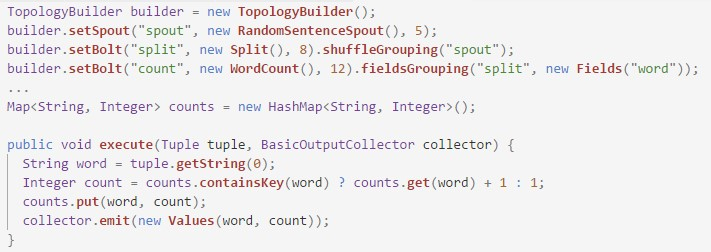
\includegraphics[width=0.95\textwidth]{img/StormAPI.jpg}
    \caption{,,Apache Storm'' žodžių skaičiavimo programos kodo pavyzdys}
    \label{fig:stormapi}
\end{figure} \par

,,Apache Storm'' parašytos programos yra žemo lygio abstrakcijos. \ref{fig:stormapi} pavyzdyje matome labai sumažintą programos pavyzdį. 
Kadangi tai yra žemo lygio programa mes turime apsirašyti visas srauto apdorojimo stadijas pažingsniui, tai yra: setSpouts(..), 
kur nustatoma duomenų įeiga ir koks bus paralelizmas, setBolt(..), kur nustatatomi apdorojimo moduliai, kokius duomenis gaus iš 
prieš tai buvusio modulio ir paralelizmas. Žemiau, execute() metodas aprašo, kaip gali atrodyti apdorojimo modulis, kuris suskaičiuoja 
kiek skirtingų žodžių pro jį praėjo. Šios architektūros programų kūriamo laikas užtruks ilgiau negu kitoms architektūroms su aukštu 
abstrakcijos lygių, tačiau žemas abstrakcijos leidžia rašyti daug greičiau veikiančias programas, kadangi programuotojas turi beveik pilną kontrolę.

\begin{figure}[!htbp]
    \centering
    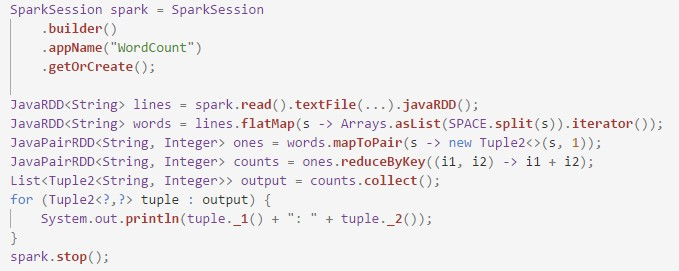
\includegraphics[width=0.95\textwidth]{img/SparkAPI.jpg}
    \caption{,,Apache Spark'' žodžių skaičiavimo programos kodo pavyzdys}
    \label{fig:sparkapi}
\end{figure} \par

,,Apache Spark'' parašytos programos yra aukšto lygio abstrakcijos. \ref{fig:sparkapi} pavyzdyje matome realu beveik išbaigtą programos pavyzdį. 
Programa aprašoma funkciškai, todėl kodo rašymas trunka daug trumpiau ir tokį kodą daug patogiau skaityti. Tačiau prarandama galimybė optimizuoti
ir paralelizmo klausimas paliekamas architektūrai, taip pat ,,Apache Spark'' yra ne pilnai srautinio, o mikro-paketinė (angl. micro-batching) 
architektūra, todėl vartotojas turi apsirašyti kokio dydžio paketais bus renkami duomenys\cite{shoro2015big}.

\begin{figure}[!htbp]
    \centering
    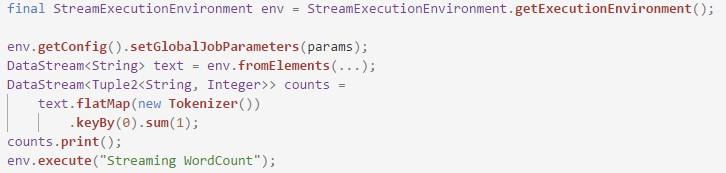
\includegraphics[width=0.95\textwidth]{img/FlinkAPI.jpg}
    \caption{,,Apache Flink'' žodžių skaičiavimo programos kodo pavyzdys}
    \label{fig:flinkapi}
\end{figure} \par

,,Apache Flink'' parašytos programos yra aukšto lygio abstrakcijos. \ref{fig:flinkapi} pavyzdyje matome pilnai veikiančios programos pavyzdį. ,,Apache Flink'' 
architektūra pati užsiema resursų distribucija, todėl programuotojui lieka tik parašyti veikianti kodą, o sistema pati susitvarkys su paralelizmu. Tačiau 
tai reiškia, kad su šia architektūra parašytos programos nepavyks optimizuoti taip pat gerai kaip žemo lygio abstrakcijos architektūros.

\subsection{Apibendrinimas}
Iš šiu triju text architektūrų reikia pasirinkti vieną, kuri labiausiai tiks rodiklių duomenų apdorojimui. Ši architektūra turi sugebėti greitai apdoroti duomenis,
prioretizuojant greiti virš tikslumo, kadangi vienas iš pagrindinių naudotojų yra statiską renkančios įstaigos, kurios gali sau leisti tam tikrą paklaidą,
ir programuotojas turi galėti aprašyti daug skirtingų sprendimų skirtingiems rodikliams.\par

\begin{center}
    \begin{table}[!htbp]
        \caption{Srautinių architektūrų palyginimas}
        \label{table:comparer}
        \begin{tabular}{ | l | c | c | c | } 
            \hline
            Charakteristika & ,,Apache Storm'' & ,,Apache Spark'' & ,,Apache Flink'' \\* \hline
            Pristatymo semantika & Bent vieną kartą & Tiksliai vieną kartą & Tiksliai vieną kartą \\* \hline
            Uždelstumas & Žemas & Aukštas & Vidutinis \\* \hline
            Pralaidumas & Žemas & Aukštas & Vidutinis \\* \hline
            Abstrakcijos lygis & Žemas & Aukštas & Aukštas \\* \hline
        \end{tabular}
    \end{table}
\end{center}\par

Kaip matome iš atliktos analizės \ref{table:comparer} lentelėje ir apsibrėžtų reikalavimų, mums labiausiai tinkanti srautinio apdorojimo architektūra yra ,,Apache Storm''. 
Nors jos pralaidumas yra žemas, mums daug aktualiau yra greitis, taip pat žemas abstarkcijos lygis leis daug geriau optimizuoti sprendimą su šia architektūra. Su ją kursime
sprendimą, kurį lyginsimę su reliacinės duomenų bazės sprendimu.

\section{Testinių duomenų generatorius}

Kad išmatuotume abiejų sistemų greitaveiką, sukurėme testinių duomenų generatorių, kuris tiktų abiems sistemos. Todėl jis yra padarytas iš dviejų dalių:
,,Apache Kafka'' žinučių sistemos ir su ,,Python'' programavimo kalba sukurtas duomenų generatorius (\ref{fig:generator} pav.).

\begin{figure}[!htbp]
    \centering
    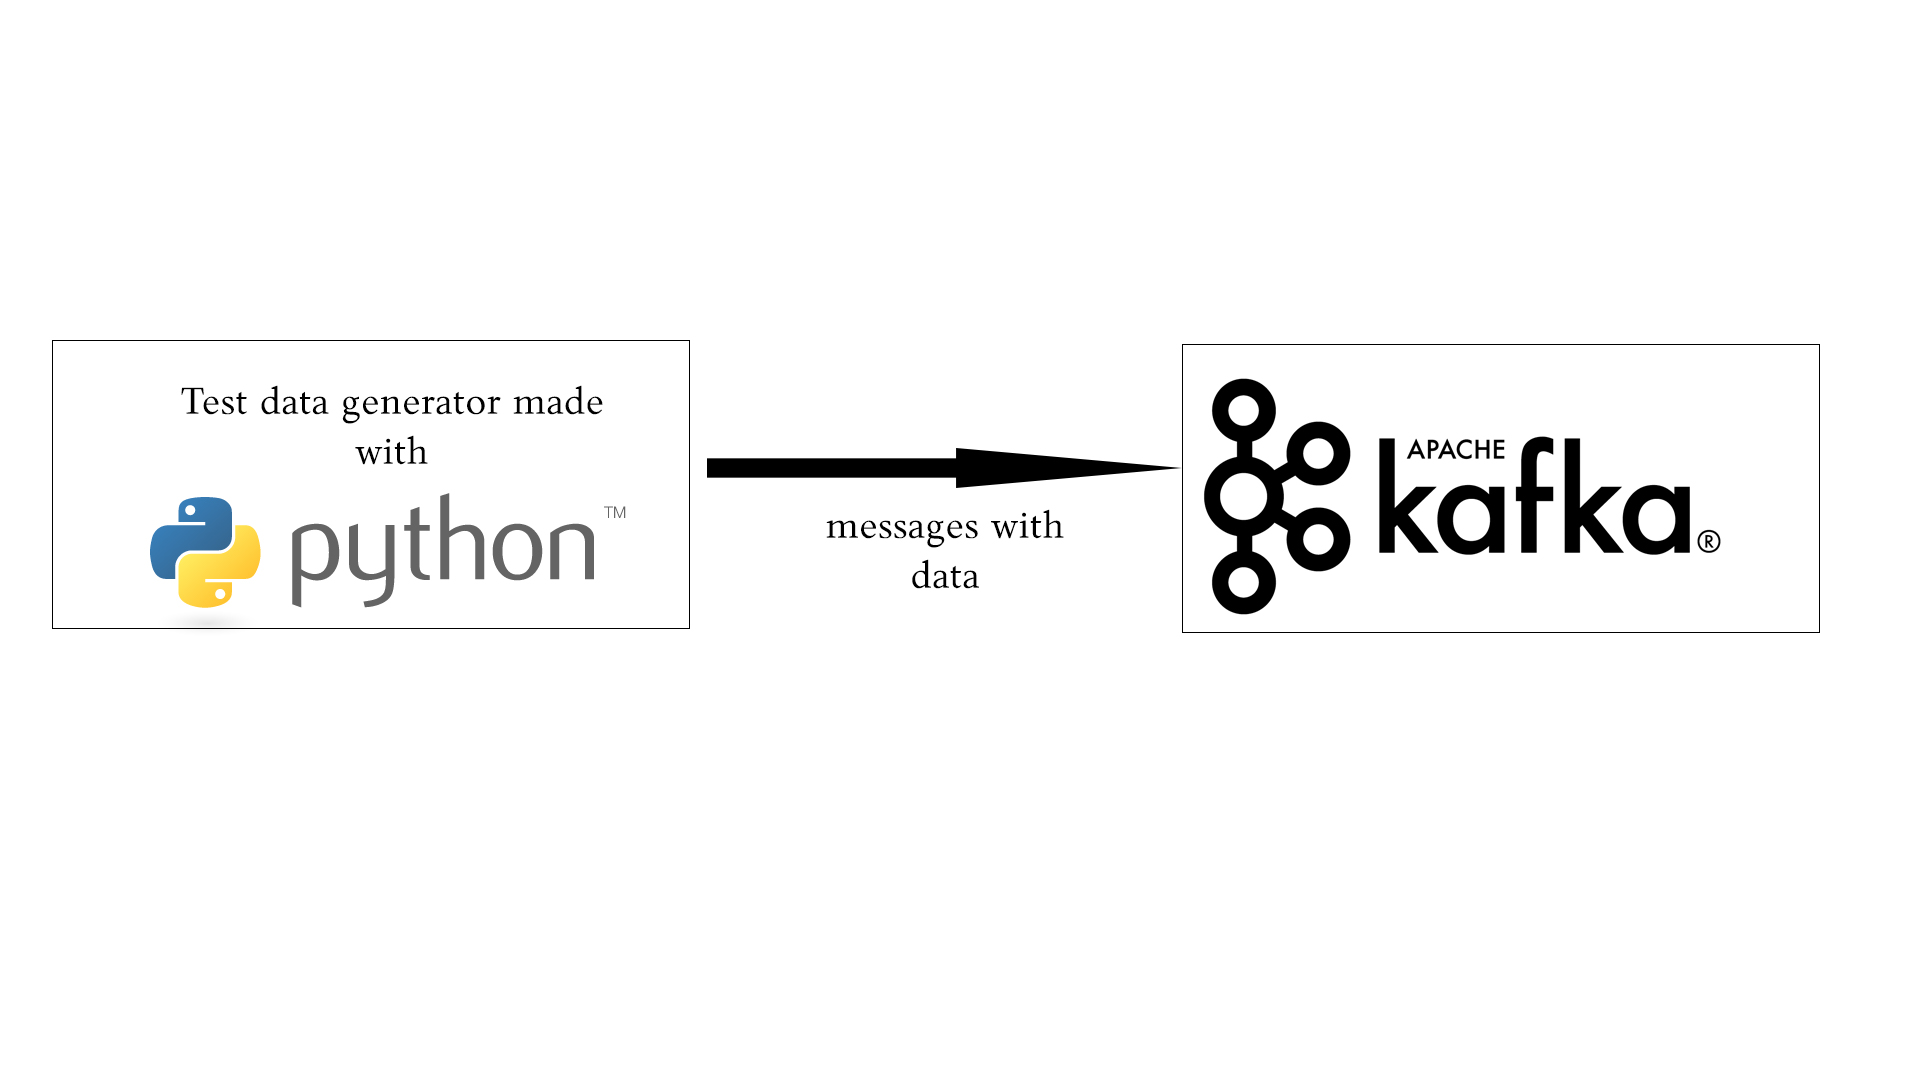
\includegraphics[width=0.95\textwidth]{img/testdatagenerator.jpg}
    \caption{Testinių duomenų generatoriaus architektūra}
    \label{fig:generator}
\end{figure}
\subsection{,,Python'' duomenų generatorius}

Su ,,Python'' kalba pararšytas generatorius, kuris sukuria didelį kiekį duomenų, naudojant ,,random'' biblioteką ir veliau po vieną siunčia į 
,,Apache Kafka'' žinučių sistemą. Kadangi bendravimas tarp programos ir žinučių sistemos yra labai greitas, testavimui įvestas kintamasis, kuris
nurodo, kiek laiko laukti iki kito siuntimo, naudojant ,,time'' bibliotekos ,,sleep'' funkciją į kurią galima įvesti laiką sekundėmis, kuris
nurodo kokiam laiko tarpui sustabdomas einamasis procesas. Tačiau, kadangi ,,sleep'' funkcija naudoja procesoriaus dažnį, ji nėra absoliučiai tiksli
ir jos paklaida priklauso nuo procesoriaus ir operacinės sistemos\cite{imtiaz20}. Todėl su atskirą ,,Python'' programą buvo išmatuotas kompiuterio,
su kurios buvo vykdomi testai, paklaida, kuri buvo 0.86 milisekundės. Derinant šį uždelsimo laika bus bandoma nustatyti abiejų sprendimu pralaidumus.

\subsection{,,Apache Kafka'' žinučių sistema}



\section{Sprendimo naudojančio relaicinę duomenų bazę testas}

\subsection{Apibūdinimas}

Kaip paruošiu sistema ir kodėl python turėtų būti pakankamai greitas sprendimas, kad netrukdytų rezultatams

\subsection{Testavimo rezultatai}

Oh shit its slow.

\section{Srautinio duomenų apdorojimo sprendimo testas}

\subsection{Apibūdinimas}

,,Apache Storm'' programa yra vadinama topologija, kuri susideda iš ,,Spout'' ir ,,Bolt'' modulių. ,,Spout'' tai modulis gaunantis duomenis
iš išorinės sistemos ir perduodantis juos į pirmą ,,Bolt'' modulį. ,,Bolt'' yra atsakingi už duomenų apdorojima ir atidavimą atgal į išorę.
Moduliai tarpusavyje perduoda duomenų ,,Tuple'' tipu, kuris laiko duomenis ir architektūros sugeneruotą identifikatorių, 
kurio pagalba užtikrina, kad duomenis sėkmingai nuėjo iki sekančio žingsnio. 
Šiam uždaviniu spresti buvo pasirinkta suskurti:
\begin{enumerate}
    \item ,,kafka-spout'' - ,,Spout'' modulis, kuris gauna duomenis iš ,,Apache Kafka'' žinučių sistemos ir perduoda juos pirmam ,,Bolt'' moduliui.
    \item ,,calculate-price-bolt'' - ,,Bolt'' modulis, kuris gauna string tipo duomenis iš ,,kafka-spout'' ir apdoroja vieną atejusį ,,Tuple''.
    \item ,,aggregate-price-bolt'' - ,,Bolt'' modulis, kuris gauta apdorota ,,Tuple'' įdeda į ,,HashMap'' tipo sąrašą ir visą sąrašą perduoda toliau.  
\end{enumerate}\par
Kadangi ,,Apache Storm'' yra žemo lygio architektūra programuotojas turi pats numatyti paralelizmo lygi kiekviename modulyje. 
Po bandymų buvo nuspresta modelių konfiguraciją daryti tokią(\ref{fig:stormtopology} pav.): ,,kafka-spout'' - 5 paralelus procesai, ,,calculate-price-bolt''
 - 5 paralelus procesai ir ,,aggregate-price-bolt'' - 1 paralelus procesas. Pakutinį moduli negalima leisti paraleliai, nes jis pas save 
 laiko bendrą sąrašą, kurio pakartotinas keitimas sugadina duomenis.\par
\begin{figure}[!htbp]
    \centering
    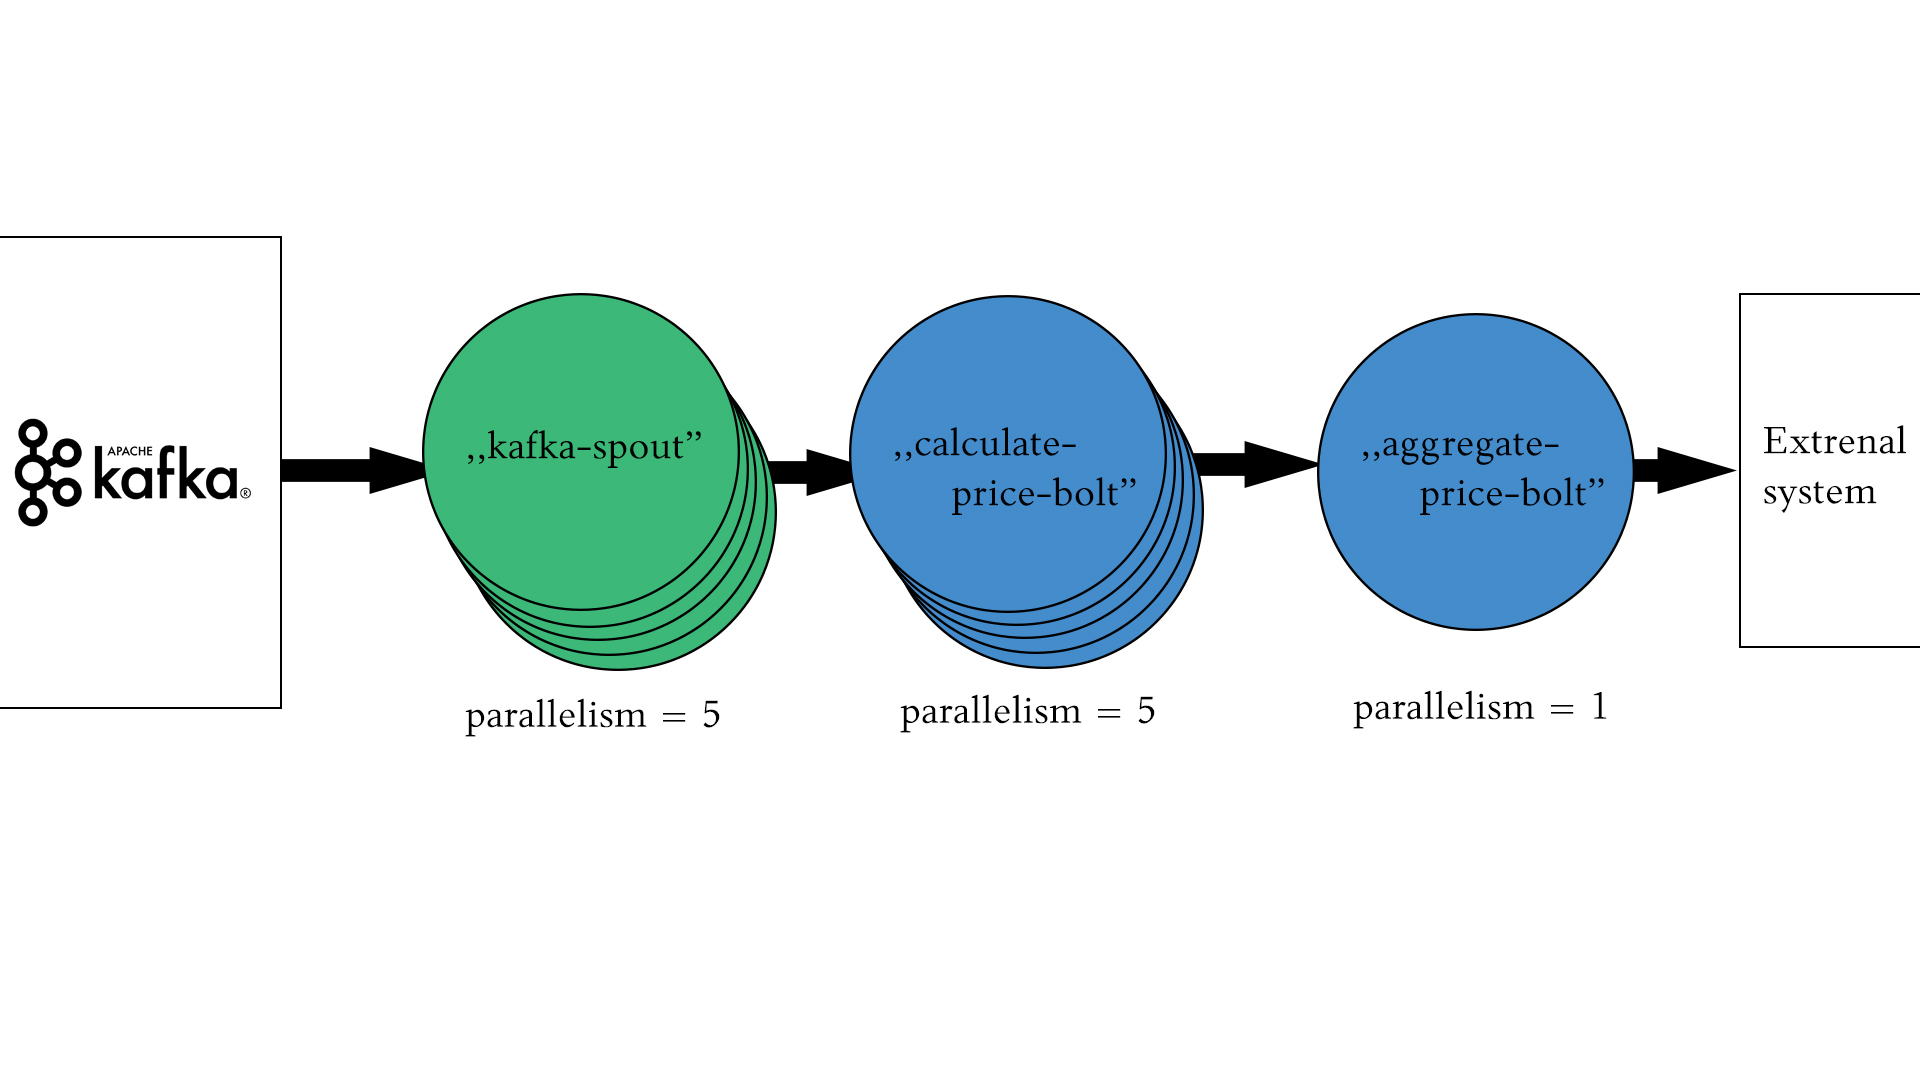
\includegraphics[width=0.95\textwidth]{img/topology.jpg}
    \caption{,,Apache Storm'' realizuota topologija}
    \label{fig:stormtopology}
\end{figure}
Prieš pradedant testavimą į sistemą buvo sugeneruota 10 milijonų įrašų, kad būtų sudarytos sąlygos panašios kaip ir reliacinei duomenų bazei.
Paleista testavimo programa siunčianti 1,5 milijono duomenų neribojant siuntimo greičio, rezultatai buvo stebimi įrašais tekstiniame dokumente.
Šiai sistemai pagal nutylejimą buvo išskirti 832 megabaitai operatyvios atminties (angl. RAM). 
\subsection{Rezultatas}
Visi duomenys buvo apdoroti per 274 sekundes, kas yra maždaug 4,5 minutės. Vidutiniška vienos operacijos trukmė - 75 milisekundės.
Lėčiausia sistemos grandis buvo ,,aggregate-price-bolt'', nes jo negalima buvo leisti paraleliai. Šios sistemos veikimą pagreitinti 
įmanoma tik perdavus paskutinio moduliu aggregavimą į sąrašą kitai architektūrai, kadangi visus kitus veiksmus galima leisti paralelei. 

\section{Experimento apibendrinimas}

\subsection{Rezultatai}

Palyginsiu srautinės ir reliacinės sprendimų pralaidumus.

\subsection{Eksperimento išvados}

Ką mes iš tu testu galime pasakyti.

\sectionnonum{Rezultatai ir išvados}
Darbo rezultatai:
\begin{itemize}
    \item Sukurtas testinių duomenų generatorius, kurio pagalba buvo vykdomas pralaidumo testavimas.
    \item Sukurtas sprendimas su pasirinkta srautinio apdorojimo architektūra.
    \item Atlikti pralaidumo testai sukurtam srautinio apdorojimo sprendimui, apibendrinti sprendimų pralaidumo testų rezultatai.
\end{itemize}

Darbo išvados:
\begin{itemize}
\item 
\item
\end{itemize}

\printbibliography[heading=bibintoc] 

\end{document}
